\section{NIST Statistical Test Suite Results}\label{app:emp_results}

% To evaluate the statistical quality of our DSphinx headers, we compare our implementation\github{} against the original Sphinx by Danezis\footnote{\url{https://github.com/UCL-InfoSec/sphinx}} using the NIST SP 800-22 statistical test suite~\cite{NIST-SP80022}.  
A detailed description of each test, its implementation, and guidance for interpreting results can be found in the NIST SP 800-22 documentation~\cite{NIST-SP80022}.  
This suite comprises the following 15 tests:
\begin{multicols}{2}  % 2 columns
\begin{enumerate}[topsep=2pt, itemsep=0pt]
     \item Frequency
     \item Block Frequency
     \item Cumulative Sums
     \item Runs
     \item Longest Run
     \item Rank
     \item Discrete Fourier Transform
     \item Non-overlapping Matchings
     \item Overlapping Matchings
     \item Universal Statistical
     \item Approximate Entropy
     \item Random Excursions
     \item Random Excursions Variant
     \item Serial
     \item Linear Complexity
\end{enumerate}
\end{multicols}

Each test produces a p-value, which quantifies how likely the observed data could be generated by a uniform source.  
For truly random headers, the distribution of p-values over many samples should be statistically uniform (Fig.~\ref{fig:hist_p-values}). 
\begin{figure}[H]
    \centering
    \includegraphics[width=\linewidth]{Appendices/hist_p-valuesV2.png}
    \caption{Distribution of p-values across all NIST SP 800-22 tests.}
    \label{fig:hist_p-values}
\end{figure}

NIST recommends interpreting these results using two complementary criteria:  
(i) the proportion of sequences that pass each test, and  
(ii) the uniformity of the p-value distributions.  

\medskip
\noindent\textbf{Passing Rate Analysis.}
Fig.~\ref{fig:proportion} highlights the proportion of sequences that passed each NIST test for both implementations.
Following NIST guidelines, the significance level is set to $\alpha = 0.01$, and the confidence interval over $n$ samples is defined as $(1 - \alpha) \pm 3 \sqrt{\frac{\alpha (1 - \alpha)}{n}} $.
% Our implementation fails only three tests: \textit{Non-overlapping Matching}, \textit{Random Excursions}, and \textit{Random Excursions Variant}, all of which are also failed by the original Sphinx implementation.  
% In contrast, DSphinx passes three tests that Sĥinx fails: \textit{Frequency}, \textit{Cumulative Sums}, and \textit{Overlapping Matching}.

\bigskip
\noindent\textbf{P-value Distribution Analysis.}
Fig.~\ref{fig:hist_p-values} shows the p-value histograms for both implementations across all 15 NIST tests.
Uniformity of these distributions is further assessed using a Chi-square goodness-of-fit test (Fig.~\ref{fig:chisquare}) with a significance threshold of $0.0001$, as recommended by NIST.
% Fig.~\ref{fig:chisquare} presents these results, highlighting that our implementation achieves uniform p-value distributions on the \textit{Frequency} and \textit{Cumulative Sums} tests, whereas the original Sphinx fails them.

\begin{figure}[H]
    \centering
    \begin{subfigure}[t]{0.46\linewidth}
        \centering
        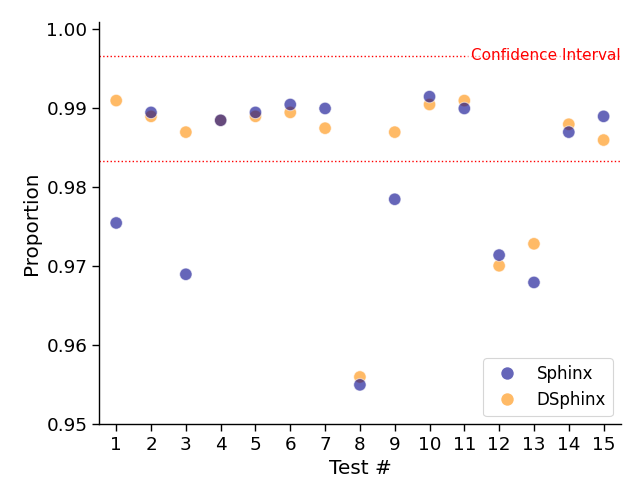
\includegraphics[width=0.95\linewidth]{Appendices/proportion_dotV2.png}
        \caption{Proportion of sequences passing each test (with significance level = 0.01).}
        \label{fig:proportion}
    \end{subfigure}
    \hfill
    \begin{subfigure}[t]{0.52\linewidth}
        \centering
        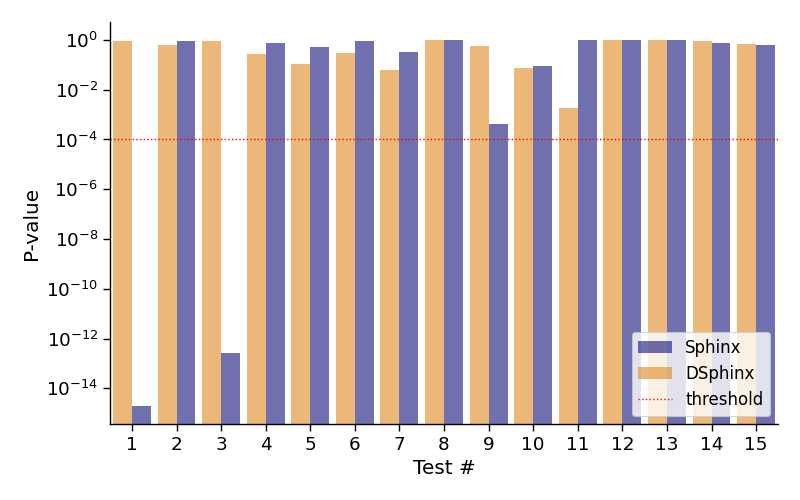
\includegraphics[width=\linewidth]{Appendices/chisquareV2.png}
        \caption{Chi-square goodness-of-fit test assessing uniformity of p-value distributions of Fig.~\ref{fig:hist_p-values}.}
        \label{fig:chisquare}
    \end{subfigure}
    \caption{Evaluation of the NIST SP 800-22 statistical randomness test suite.}
    \label{fig:nist-results}
\end{figure}
